
\begin{figure*}[t]
    \centering
    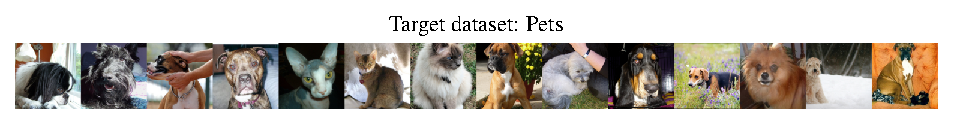
\includegraphics[width=\linewidth]{figures/pets_targets.pdf}\\
    \vspace{-0.1in}
    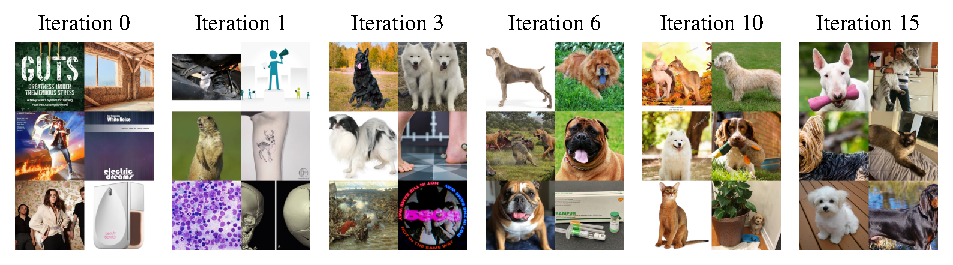
\includegraphics[width=\linewidth]{figures/pets-progression-962-2col-3row.pdf}
    % 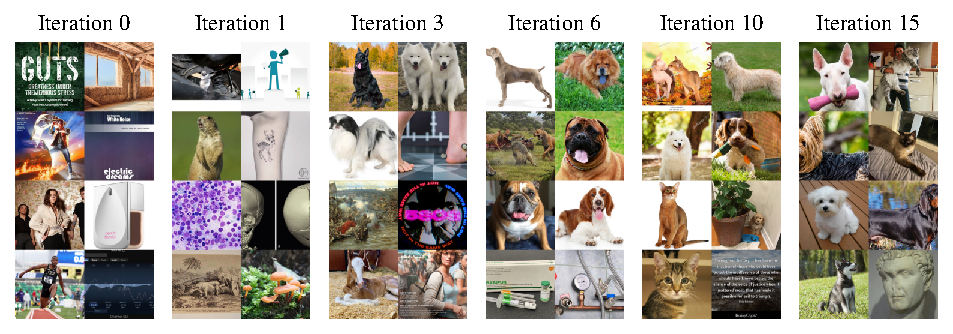
\includegraphics[width=\linewidth]{figures/pets-progression-962-2col.pdf}
    \vspace{-0.28in}
    \caption{
    % \textbf{Progression of downloaded images over training.} The top row shows the target distribution and the bottom ones show the sets of images queried by our Internet Explorer. As the progression goes on, the image set discovered by the Internet Explorer starts to more closely resemble the target dataset distribution.
    \textbf{Progression of downloaded images across training.} \textbf{Top:} samples of Oxford-IIIT Pets images. \textbf{Bottom:} samples of images queried by Internet Explorer across iterations. As it learns, it makes queries that are progressively more relevant to the target dataset.
    }
    \label{fig:progression}
    \vspace{-0.15in}
\end{figure*}

\section{Results and Analysis}
\subsection{Self-supervised Results}
Figure~\ref{fig:learning_curves} shows how Internet Explorer improves the $k$-NN accuracy more efficiently than sampling queries uniformly at random from the concept vocabulary. In fact, random sampling occasionally decreases accuracy, likely due to the fact that Internet images can generally be unsuitable for pre-training due to issues such as watermarks, images containing text, and overly photogenic images~\cite{mezuman2012learning,chen2015webly}. Table~\ref{tab:main_results} shows that our method significantly improves on the starting MoCo-v3 (ImageNet + target) checkpoint and can outperform a CLIP~\cite{radford2021learning} model of the same size while using much less compute and data. This is impressive as CLIP can be thought of as an oracle, since its training set contains up to 20k Bing image search results for each WordNet lemma (in addition to other queries).
Using GPT-generated descriptors in ``Ours++'' also significantly improves performance by enabling Internet Explorer to generate diverse views of the most useful concepts. 
% We show example image results with and without descriptors in the supplementary. 

\subsection{Self-supervised Exploration Behavior}
Figure~\ref{fig:reward_over_training} shows the progression of Internet Explorer (Ours++) behavior on the Pets dataset in the self-supervised setting. Since Pets consists of cat and dog breeds, to analyze the results, we use the WordNet hierarchy to divide concepts in our vocabulary into 5 meaningful categories: cats, dogs, non-cat felines (e.g., lion), non-dog canines (e.g., wolf), and other. This categorization is only done for this post hoc analysis and is not provided during training. Figure~\ref{fig:reward_over_training} (top) shows that
% the average estimated reward within each category across the first 20 iterations of training, and the bottom one shows how much probability mass each category has. 
Internet Explorer rapidly identifies the roughly $0.3\%$ of concepts that are useful for Pets. During the first two iterations, the average estimated reward for each category is roughly the same. However, after the first dog concept is searched in iteration $\#2$, the estimated reward and probability mass for dogs and other canines rapidly increases. The same happens for cats after the first cat is searched in iteration $\#4$. Interestingly, while ``other felines'' and ``other canines''  have higher average reward than the ``other'' category, they still have much lower reward than cats and dogs. This indicates that our model understands that other felines and canines (mostly large, wild predators) are only moderately relevant for house pet cats and dogs. 

Figure~\ref{fig:progression} shows how Internet Explorer downloads progressively more useful images over time. It shows 8 random images that were downloaded in iteration $\#0$, $\#1$, $\#3$, $\#6$, $\#10$, and $\#15$. Iteration $\#0$ contains mostly useless data, like graphics or screenshots, but Pets-relevant images already make up most of the downloads by iteration $\#3$. 


\begin{figure*}[t]
    \centering
    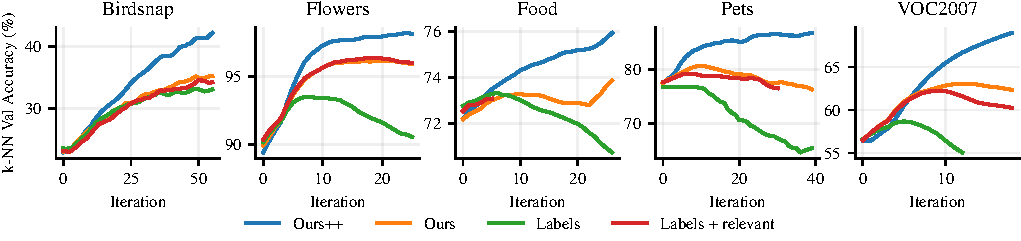
\includegraphics[width=\linewidth]{figures/semisup-curves-updated.pdf}
    \vspace{-0.3in}
    \caption{\textbf{Learning curves in label set-guided setting.} Using knowledge of the label set improves the performance of all methods. }
    \label{fig:semisup_learning_curves}
    % \vspace{-0.05in}
\end{figure*}


\subsection{Label Set-guided Results}
% As discussed earlier, we now make use of the label set of the target dataset without knowing the exact image-label mapping. 
Internet Explorer significantly outperforms the stronger baselines in the label set-guided setting where we additionally have knowledge of the label set. Searching for the label set continuously provides useful data and helps us rapidly identify other useful concepts. Together with the diversity promoted by GPT descriptors, Ours++ outperforms CLIP in 3/5 datasets and approaches its performance in the other 2, using just 2.5\% of the time and 0.5\% the data.
% Note that we train Internet Explorer from scratch on VOC2007 and do not use an ImageNet pre-trained MoCo-v3 model as initialization. 
% Note that we train from scratch on VOC2007 and do not do ImageNet pre-training because ImageNet's similarity to VOC2007 obscures the effect of Internet Explorer.

\subsection{Learning from other sources of data}
\label{subsec:search_engine_main}
\begin{table*}[t]
    \centering
    \begin{adjustbox}{width=1\textwidth}
    \begin{tabular}{@{\extracolsep{4pt}}lccccccccc}
    \toprule
        % Model & Flowers102 & Food101 & Stanford Cars & Oxford-IIIT Pets & Total Images & GPU-hours \\
        \multirow{2}{*}{\textbf{Model}}
        &\multicolumn{3}{c}{\textbf{Flowers}} 
        &\multicolumn{3}{c}{\textbf{Food}}
        &\multicolumn{3}{c}{\textbf{Pets}} \\
        \cmidrule{2-4} \cmidrule{5-7} \cmidrule{8-10}
        
        
        & Google & Flickr & LAION & Google & Flickr & LAION & Google & Flickr & LAION \\
    \midrule
    \textit{Fixed dataset} &&&&&&&&&\\    
        \;\;\; MoCo-v3 (IN)                          & $83.2$ & $83.2$ & $83.2$ & $70.5$ & $70.5$ & $70.5$ & $79.6$ & $79.6$ & $79.6$ \\
        \;\;\; MoCo-v3 (IN + target)                 & $94.6$ & $94.6$ & $94.6$ & $78.3$ & $78.3$ & $78.3$ & $85.3$ & $85.3$ & $85.3$ \\
    \midrule
    \textit{Undirected search} &&&&&&&&&\\    
        \;\;\;Random exploration                     &  $95.3$  &  $95.2$  &  $94.8$  &  $77.0$ &  $80.0$  &  $80.2$  &  $85.6$ & $84.4$  & $85.1$ \\
    \midrule 
    \textit{Internet Explorer} &&&&&&&&&\\    
        % \;\;\;Random exploration                      &    &    &    &    &    &    &    &    &    \\
        % \;\;\;Ours                                   &  ? &  ? &  ? &  ? &  ? \\
        \;\;\;Ours++ (no label set)                  &  $98.4$  &  $98.1$  &  $94.6$  &  $81.2$  &  $80.3$  &  $80.9$  &  $87.3$  &  $88.4$  &  $85.9$  \\
    % \midrule 
        % \;\;\;Search labels only                      &  ? &  ? &  ? &  ? &  ? \\
        % \;\;\;Labels + relevant                       &    &    &    &    &    &    &    &    &    \\
        % \;\;\;Ours                                    &  ? &  ? &  ? &  ? &  ? \\
        \;\;\;Ours++ (with label set)                &  $\bf{99.1}$ &  $\bf{99.0}$ &  $\bf{95.8}$ & $\bf{84.6}$ & $\bf{81.9}$  &  $\bf{81.0}$  & $\bf{90.8}$ &  $\bf{89.1}$  &  $\bf{86.7}$  \\
    \bottomrule
    \end{tabular}
    \end{adjustbox}
    \vspace{-0.1in}
    \caption{\textbf{Linear probe accuracy with other search engines}. Internet Explorer improves its performance using any search engine, including Flickr and our custom text-based LAION search engine.}
    \label{tab:search_engine}
\end{table*}

We primarily obtain images by querying Google Images, but Internet Explorer is compatible with any text-to-image search engine. To measure the effect of the choice of search engine, we also test Internet Explorer with the Flickr photo search API and a custom search engine we built on top of a subset of LAION-5B~\cite{schuhmann2022laion}. LAION-5B consists of noisy web-scraped (text, image) pairs, and our custom LAION search engine searches using approximate nearest neighbors in \textit{text embedding space}. Thus, it tests whether Internet Explorer can still improve even when the search engine has little inductive bias. We discuss more details in Appendix~\ref{sec:search_engine_details}. \cref{tab:search_engine} shows that Internet Explorer consistently improves over time, regardless of the search engine we use. Google consistently does best, followed by Flickr, then LAION (which has the smallest pool of images to draw from). Using Internet Explorer to search LAION-5B consistently performs \textit{better} than random exploration---indicating that Internet Explorer is effective even for selecting data from a static dataset. 
% Overall, these results are a proof of concept that Internet Explorer can efficiently utilize any window into the Internet's vast ocean of image data. 



\subsection{Effect of image reward type}
\label{subsec:reward_analysis}
We run an ablation on the type of image relevance reward. Instead of calculating the image reward based on the average similarity to the $k=15$ nearest neighbors in representation space (as in \cref{subsec:ssl}), we also try using $k=1$ or the MoCo contrastive loss as the reward. Table~\ref{tab:image_reward} compares these three metrics in the label set-guided setting and shows that $k=15$ does best. We explain this result by qualitatively comparing the behavior of various metrics on Food101 in \cref{fig:reward_ranking} in the appendix. The MoCo loss does not identify relevant concepts, instead preferring images that are difficult to align across augmentations. Representation similarity with $k=1$ also fails, as it prefers images of zebras and text because these images are highly similar to a few outlier images in Food101. Our proposed reward with $k=15$ eliminates the influence of outliers and avoids this problem.


% \subsection{Do we rely on Google's multimodal knowledge?}
% \begin{table}[]
%     \centering
%     \begin{tabular}{lcc}
%         \toprule
%         Search Engine & Pets (with label set) \\
%         \midrule
%         LAION 400M w/ text sim &  running \\
%         Google Images & have $\#$ \\
%         \bottomrule
%     \end{tabular}
%     \caption{\textbf{Replacing Google Images with text-only search.} }
%     \label{tab:search_engine}
% \end{table}


% \begin{wraptable}{r}{0.5\linewidth}
%     \centering
%     \begin{tabular}{lcc}
%         \toprule
%         Reward Type & Food \\
%         \midrule
%         MoCo loss & 81.2 \\
%         1-NN sim  & 83.2 \\
%         15-NN sim (ours) & \textbf{84.6} \\
%         \bottomrule
%     \end{tabular}
%     \caption{\textbf{Ablation on type of image reward.}
%     % We compare LP accuracy of 3 different rewards on Food in the label set-guided setting.
%     MoCo loss does not identify relevant concepts, and $k=1$ similarity is too noisy to identify useful concepts. }
%     \label{tab:image_reward}
% \end{wraptable}

\begin{table}[h]
    \centering
    \begin{tabular}{lcc}
        \toprule
        Reward Type & Food \\
        \midrule
        MoCo loss & 81.2 \\
        1-NN sim  & 83.2 \\
        15-NN sim (ours) & \textbf{84.6} \\
        \bottomrule
    \end{tabular}
    \caption{\textbf{Ablation on type of image reward.}
    % We compare LP accuracy of 3 different rewards on Food in the label set-guided setting.
    MoCo loss does not identify relevant concepts, and $k=1$ similarity is too noisy to identify useful concepts. }
    \label{tab:image_reward}
\end{table}


%%% Local Variables:
%%% coding: utf-8
%%% mode: latex
%%% TeX-engine: xetex
%%% TeX-master: "../thesis"
%%% End:
